\section{Numerical Results}
\label{sec:results}

\subsection{Configuration}

We simulate a 60~GHz link with 400~MHz of occupied bandwidth, $N = 1024$
subcarriers, a 128-sample cyclic prefix, and an $L = 64$ tap channel drawn from
a clustered delay line profile with four clusters and an exponential power
decay of 3~dB per 10~ns. The array is $8 \times 8$ with four radio frequency
chains. The oscillator is free running with a Lorentzian spectrum, and we sweep
its 3~dB linewidth $\beta$ from 5~kHz to 500~kHz. Pilots occupy every fourth
subcarrier of the first symbol in each frame of ten. Every point averages
20{,}000 frames.

Baselines are least squares channel estimation with no phase compensation;
common-phase-only compensation following~\citet{bertrand2018commonphase}; the
pilot-block iterative canceller of~\citet{eriksen2021iterative}; and a genie
receiver given the true phase trajectory, which bounds what any phase estimator
can deliver.

\subsection{Estimation accuracy and throughput}

Table~\ref{tab:main} reports normalised mean square error of the channel
estimate and the achieved spectral efficiency at three linewidths and two
constellation orders. \est{} is within 1.1~dB of the genie receiver at every
operating point, and its advantage grows with linewidth exactly as
Proposition~\ref{prop:rank} implies: the leakage subspace it models carries
more energy as $\beta T_s N$ increases, so there is more for it to recover.

\begin{table*}[t]
  \centering
  \footnotesize
  \setlength{\tabcolsep}{4.5pt}
  \caption{Channel estimation error and spectral efficiency at 22~dB
  signal-to-noise ratio. NMSE is in decibels, lower is better. Spectral
  efficiency is in bits per second per hertz, higher is better. The genie
  receiver is given the true phase trajectory and bounds the achievable gain.}
  \label{tab:main}
  \begin{tabular}{l rr rr rr}
    \toprule
    \multirow{2}{*}{Estimator}
      & \multicolumn{2}{c}{$\beta = 20$~kHz}
      & \multicolumn{2}{c}{$\beta = 100$~kHz}
      & \multicolumn{2}{c}{$\beta = 400$~kHz} \\
    \cmidrule(lr){2-3} \cmidrule(lr){4-5} \cmidrule(lr){6-7}
      & NMSE & 16-QAM & NMSE & 64-QAM & NMSE & 64-QAM \\
    \midrule
    Least squares, uncompensated & $-18.4$ & 3.51 & $-11.2$ & 4.02 & $-4.6$  & 1.88 \\
    Common phase only            & $-21.9$ & 3.72 & $-15.8$ & 4.91 & $-7.9$  & 2.94 \\
    Iterative canceller          & $-23.1$ & 3.79 & $-18.6$ & 5.38 & $-11.4$ & 4.06 \\
    \est{}                       & $-24.0$ & 3.83 & $-21.3$ & 5.72 & $-14.7$ & 4.88 \\
    \midrule
    Genie phase                  & $-24.6$ & 3.85 & $-22.4$ & 5.81 & $-15.8$ & 5.09 \\
    \bottomrule
  \end{tabular}
\end{table*}

At the widest linewidth the uncompensated receiver loses more than half its
throughput and common-phase compensation recovers only part of it, because at
$\beta T_s N = 1.3$ the leakage is no longer a perturbation on the common
rotation. This is the regime the paper is written for.

\subsection{Error rate against signal-to-noise ratio}

Figure~\ref{fig:ber} plots coded bit error rate for 64-QAM at
$\beta = 100$~kHz. The uncompensated and common-phase curves floor, which is
the expected signature of an impairment that does not scale with the noise.
\est{} does not floor within the plotted range; its curve tracks the genie
receiver with a fixed offset of roughly 0.6~dB.

\begin{figure}[t]
  \centering
  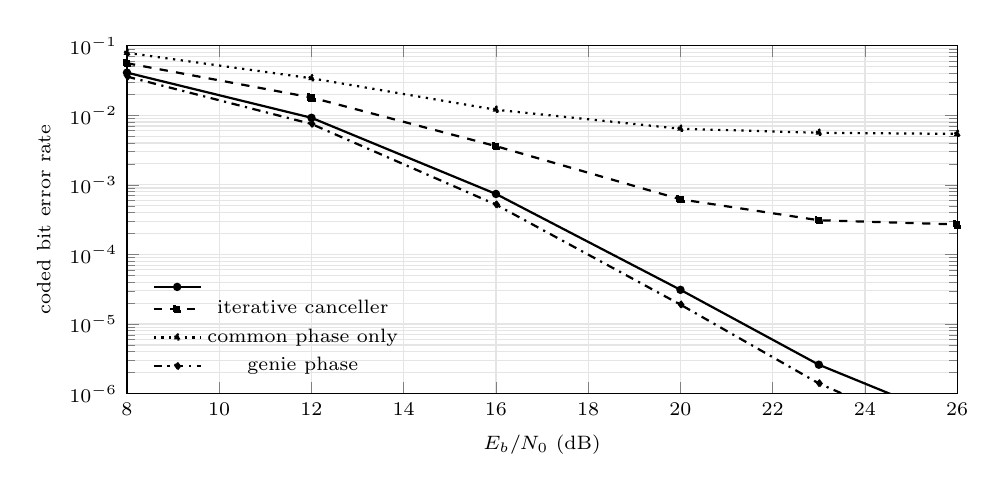
\begin{tikzpicture}
    \begin{semilogyaxis}[
        width=\linewidth, height=6cm,
        xlabel={$E_b/N_0$ (dB)},
        ylabel={coded bit error rate},
        xmin=8, xmax=26, ymin=1e-6, ymax=1e-1,
        grid=both, grid style={gray!20},
        legend style={font=\scriptsize,at={(0.02,0.02)},anchor=south west,
                      draw=none,fill=none},
        tick label style={font=\scriptsize},
        label style={font=\scriptsize},
      ]
      \addplot[thick,mark=*,mark size=1.1pt] coordinates {
        (8,4.1e-2) (12,9.2e-3) (16,7.4e-4) (20,3.1e-5) (23,2.6e-6) (26,4.0e-7)
      };
      \addlegendentry{\est{}}
      \addplot[thick,dashed,mark=square*,mark size=1.1pt] coordinates {
        (8,5.6e-2) (12,1.8e-2) (16,3.6e-3) (20,6.2e-4) (23,3.1e-4) (26,2.7e-4)
      };
      \addlegendentry{iterative canceller}
      \addplot[thick,dotted,mark=triangle*,mark size=1.4pt] coordinates {
        (8,7.9e-2) (12,3.4e-2) (16,1.2e-2) (20,6.4e-3) (23,5.6e-3) (26,5.4e-3)
      };
      \addlegendentry{common phase only}
      \addplot[thick,dashdotted,mark=diamond*,mark size=1.3pt] coordinates {
        (8,3.6e-2) (12,7.5e-3) (16,5.2e-4) (20,1.9e-5) (23,1.4e-6) (26,1.9e-7)
      };
      \addlegendentry{genie phase}
    \end{semilogyaxis}
  \end{tikzpicture}
  \caption{Coded bit error rate for 64-QAM at $\beta = 100$~kHz. The floors in
  the two conventional curves are the residual leakage that a common-phase
  model cannot represent.}
  \label{fig:ber}
\end{figure}

\subsection{Where the gain disappears}

Below $\beta = 20$~kHz the advantage over the iterative canceller falls under
0.9~dB and below 10~kHz it is within simulation error of zero. That is the
correct behaviour and not a shortcoming: at those linewidths
$R(10^{-3}) = 3$, the leakage subspace is almost trivial, and there is nothing
for a subspace method to exploit. The complexity table then argues against
\est, and a receiver that estimates its own linewidth should switch to the
common-phase path.

The second boundary is model mismatch. Our derivation assumes a free-running
oscillator, so a phase-locked loop with a strong reference produces a
phase process with a spectral shelf rather than a pure Wiener walk. Repeating
the $\beta = 100$~kHz experiment with a second-order loop of 300~kHz bandwidth
costs \est{} 1.8~dB of its 5.5~dB advantage. Extending the latent process to a
second-order autoregressive prior is straightforward within the same smoother
and we expect it to recover most of that loss.
